% Class project report: progress so far on the US Housing Crisis Analysis.
% Build: latexmk -pdf report.tex   (figures are read from ../figures/)
\documentclass[11pt]{article}

\usepackage[margin=1in]{geometry}
\usepackage[T1]{fontenc}
\usepackage{lmodern}
\usepackage{amsmath}
\usepackage{booktabs}
\usepackage{array}
\usepackage{graphicx}
\usepackage{float}
\usepackage[font=small,labelfont=bf]{caption}
\usepackage{enumitem}
\usepackage{xurl}
\usepackage[hidelinks]{hyperref}

\graphicspath{{../figures/}}
\setlist{itemsep=2pt, topsep=4pt}
% let figures share a page with text instead of floating to pages of their own
\renewcommand{\topfraction}{0.9}
\renewcommand{\bottomfraction}{0.8}
\renewcommand{\textfraction}{0.07}
\renewcommand{\floatpagefraction}{0.85}

% ---- Edit these -------------------------------------------------------------
\newcommand{\studentname}{Lucas Rubin}
\newcommand{\coursename}{DATA320}
\newcommand{\reportdate}{October 2026}
% -----------------------------------------------------------------------------

\title{Has US Population Growth Stopped Following Income?\\[4pt]
\large Income, migration and the stalling of big cities, 1880--2020\\
(progress report)}
\author{\studentname\\ \coursename}
\date{\reportdate}

\begin{document}
\maketitle

\begin{abstract}
For most of US history, population grew fastest in the states where incomes were highest. This
project asks whether that is still true and, if not, when it changed. With yearly state population
and income data from 1929 to 2024 (and decade data back to 1880 for context), I estimate how much
faster richer states grew than poorer ones, and I test whether that relationship was the same before
1970 and after 1990. It was not: before 1970 a state with 10\% higher income grew about 1.7
percentage points faster per decade, while from 1990 on income no longer predicted growth. The
difference is statistically significant ($\chi^2(1) = 19.0$), and it stays significant after
accounting for the fact that the cut years were chosen by searching the same data ($p \approx
0.001$). Exactly when the change happened is not settled. In decade data from 1950, nearly all of the
decline is in estimated net migration rather than in births and deaths. A second analysis of 81
large metropolitan areas shows that when the old big cities fell well behind US growth in 1950--70,
their metro areas mostly kept growing. Only from the 1970s did whole metro areas fall behind, almost
all of them in the Northeast and Midwest. The next stage of the project will test whether housing
costs and land-use rules explain these patterns.
\end{abstract}

% =============================================================================
\section{Questions}

Housing has become expensive in the US cities with the strongest economies. One explanation is that
rules limiting new housing keep people from moving to those cities. Before testing that
explanation, the project first establishes the basic facts it has to explain. This report covers
two of them:

\begin{enumerate}[label=\textbf{Q\arabic*.}]
  \item \textbf{Does population still grow faster in richer states, and when did that change?}
        If housing limits are keeping people out of high-income places, the historical tendency of
        population to grow toward higher incomes should have weakened.
  \item \textbf{When big cities stopped growing after 1950, did their whole region stop growing, or
        did only the city proper fall behind while its suburbs kept growing?} City population counts
        alone can make a growing region look like it is in decline.
\end{enumerate}

% =============================================================================
\section{Data}

All data are public. Table~\ref{tab:data} lists the sources. The data pipeline is written in
Python; it downloads or reads each source, converts it into one common long format, checks it and
builds the analysis panels.

\begin{table}[htbp]
\centering\small
\caption{Data sources.}
\label{tab:data}
\begin{tabular}{>{\raggedright\arraybackslash}p{0.36\textwidth}>{\raggedright\arraybackslash}p{0.33\textwidth}>{\raggedright\arraybackslash}p{0.22\textwidth}}
\toprule
Data & Source & Coverage \\
\midrule
State population & US Census via IPUMS NHGIS \cite{nhgis} & 1880--2020, every 10 years \\
State income per person & Klein \cite{klein}; Easterlin \cite{easterlin}; BEA & 1880--1920; BEA 1929 on \\
State population and income, every year & Bureau of Economic Analysis (BEA) & 1929--2024 \\
County net migration & UW--Madison Applied Population Lab \cite{apl}; ICPSR & 1950s--2010s, by decade \\
City population & Stanford CESTA \cite{cesta}; IPUMS NHGIS & 1900--2020 \\
City land area & Census Working Paper 27 \cite{gibson}; Census Gazetteer files & 1950--2020 \\
Metro areas (counties in each) & OMB 2023 metro definitions & held fixed for all years \\
\bottomrule
\end{tabular}
\end{table}

There are 50 states plus DC. A \emph{metro} is a 2023 metropolitan area, built from its
counties, so its boundary stays the same in every year. The city analysis uses the \textbf{81 metros
that contained one of the 100 largest US cities in 1950}; ``the city'' is that metro's largest 1950
city.

% =============================================================================
\section{Methods}

\subsection{How strongly does growth follow income?}

For each period, I regress population growth on income:
\begin{equation}
\underbrace{\ln P_{i,t+1} - \ln P_{i,t}}_{\text{growth of state } i}
  \;=\; \alpha_t \;+\; \beta \cdot \underbrace{\ln(\text{income per person})_{i,t}}_{\text{how rich state } i \text{ is}}
  \;+\; \varepsilon_{i,t}.
\label{eq:basic}
\end{equation}
Here $t$ is a year in the yearly data and a census year in the decade data (so $t+1$ is ten years
later). The slope $\beta$ measures how much faster richer states grow. All slopes in this report are
scaled to growth \emph{over ten years}: yearly slopes are multiplied by 10. For example,
$\beta = 0.174$ means that a state with 10\% higher income grows about
$0.174 \times \ln(1.1) \approx 0.017$, or 1.7 percentage points, faster per decade. A positive
$\beta$ means population grows faster where incomes are higher. A $\beta$ near zero means growth no
longer depends on income. The term $\alpha_t$ is a separate intercept for each year. It absorbs
anything that hit the whole country at once, such as the baby boom, wars and recessions, so $\beta$
compares states only with each other in the same year. Every state counts equally, whatever its
population.

\subsection{The statistical test}

\paragraph{Model.} I use the yearly BEA data (1929--2024) and let the slope differ across three
periods:
\begin{equation}
g_{i,t} = \alpha_t + \beta_{\text{before}}\, x_{i,t}\,\mathbf{1}[t<1970]
        + \beta_{\text{middle}}\, x_{i,t}\,\mathbf{1}[1970 \le t < 1990]
        + \beta_{\text{after}}\, x_{i,t}\,\mathbf{1}[t \ge 1990] + \varepsilon_{i,t},
\label{eq:test}
\end{equation}
where $g_{i,t}$ is growth from year $t$ to $t+1$ and $x_{i,t}$ is log income per person. The
symbol $\mathbf{1}[\cdot]$ is the \emph{indicator function}: it equals 1 when the condition in
brackets is true and 0 when it is false,
\[
\mathbf{1}[t < 1970] =
\begin{cases}
1 & \text{if } t < 1970,\\
0 & \text{otherwise.}
\end{cases}
\]
In any given year exactly one of the three indicators equals 1, so each year's growth is
explained by one slope only. For example, in 1955 the equation reduces to
$g_{i,1955} = \alpha_{1955} + \beta_{\text{before}}\, x_{i,1955} + \varepsilon_{i,1955}$. There are
4,803 state-years: 51 states (including DC), growth years 1929--2023. The 1970 and 1990 cut points
come from earlier break-date searches in this project on these same data. Because the cuts were
chosen by looking at the data, the $p$-value of this test is \emph{nominal}: it overstates the
evidence. A second test, described below, accounts for the search.

\paragraph{Hypotheses.}
\[
H_0:\; \beta_{\text{before}} = \beta_{\text{after}}
\qquad\text{vs.}\qquad
H_1:\; \beta_{\text{before}} \ne \beta_{\text{after}}.
\]

\paragraph{Test statistic.} A Wald test:
\[
W = \frac{(\hat\beta_{\text{before}} - \hat\beta_{\text{after}})^2}
         {\widehat{\operatorname{Var}}(\hat\beta_{\text{before}} - \hat\beta_{\text{after}})}
\;\sim\; \chi^2(1) \text{ under } H_0 .
\]
The variance is \emph{clustered by state}. The same state appears up to 95 times, and its yearly errors
are not independent: a state that grows quickly one year tends to grow quickly the next. Treating
the 4,803 rows as independent would make the test too confident. Clustering treats each state's
whole history as one independent unit, so there are effectively 51 observations, and it also
allows the error variance to differ across states. It does not allow for shocks shared by
neighbouring states. The significance level is $\alpha = 0.05$.

\paragraph{Accounting for the choice of cut years.} The \emph{sup-Wald} test (Andrews
\cite{andrews}) fits a model with a single break and tries every possible break year, leaving out
the first and last 15\% of years. It takes the largest Wald statistic over all those years and
compares it with the distribution of that maximum when there is no break. Because it pays for
having searched, its $p$-value is valid even though the break year was chosen from the data.

\subsection{Where the change comes from}
Over a decade, a state's growth is the sum of net migration and natural increase (births minus
deaths). Net migration comes from published county estimates, summed to states. These are
\emph{residual} estimates: each county's population change minus its recorded births and deaths.
They include immigrants from abroad. The rest of growth, total growth minus net migration, is
mostly natural increase. From the 1970s on it also absorbs any change in how completely the census
counted people; for the 1950s--60s that change sits in net migration instead. Because regression is
linear in the outcome, $\beta$ for total growth splits exactly into $\beta$ for net migration plus
$\beta$ for the rest. To make the parts add up exactly, these decade slopes use ten-year percent
change rather than log growth. Percent change gives somewhat larger slopes than the log growth in
equation~(\ref{eq:basic}): 0.35 against 0.28 in the 1950s.

\subsection{Cities versus their metros}
\label{sec:citymetro}
For each metro and each period (1950--70, 1970--90, 1990--2020), I ask whether the city and the
whole metro \emph{kept up}, meaning they grew by at least half as much as the US did over the same
period. US growth was 34\% in 1950--70, 22\% in 1970--90 and 33\% in 1990--2020. Each metro then
falls into one of four classes:

\begin{center}\small
\begin{tabular}{lll}
\toprule
& \textbf{Metro kept up} & \textbf{Metro fell behind} \\
\midrule
\textbf{City kept up}      & growing        & city-led \\
\textbf{City fell behind}  & suburbanizing  & stagnant \\
\bottomrule
\end{tabular}
\end{center}

\noindent \emph{Suburbanizing} means the city fell behind while its metro kept up. The labels
describe population counts; they do not show that anyone moved out of the city. \emph{Stagnant}
means the whole metro fell behind. A city is \emph{annexing} if its land area grew more than 20\%
over the period (a merger with its county also counts), so new residents partly came from moving the
city line; otherwise it has \emph{fixed} boundaries. Ranges around each share come from the
bootstrap: I resample the metros with replacement 999 times and report the middle 90\% of the
results. The 81 metros are not a random sample but all metros with a 1950 top-100 city, so a range
shows how much a share depends on which metros are in the set. The decision rules (what share
counts as ``mostly suburbanization,'' and so on) were written down before any class or share was
computed.

% =============================================================================
\section{Results}

\subsection{Growth stopped following income (Q1)}

\begin{figure}[htbp]
\centering
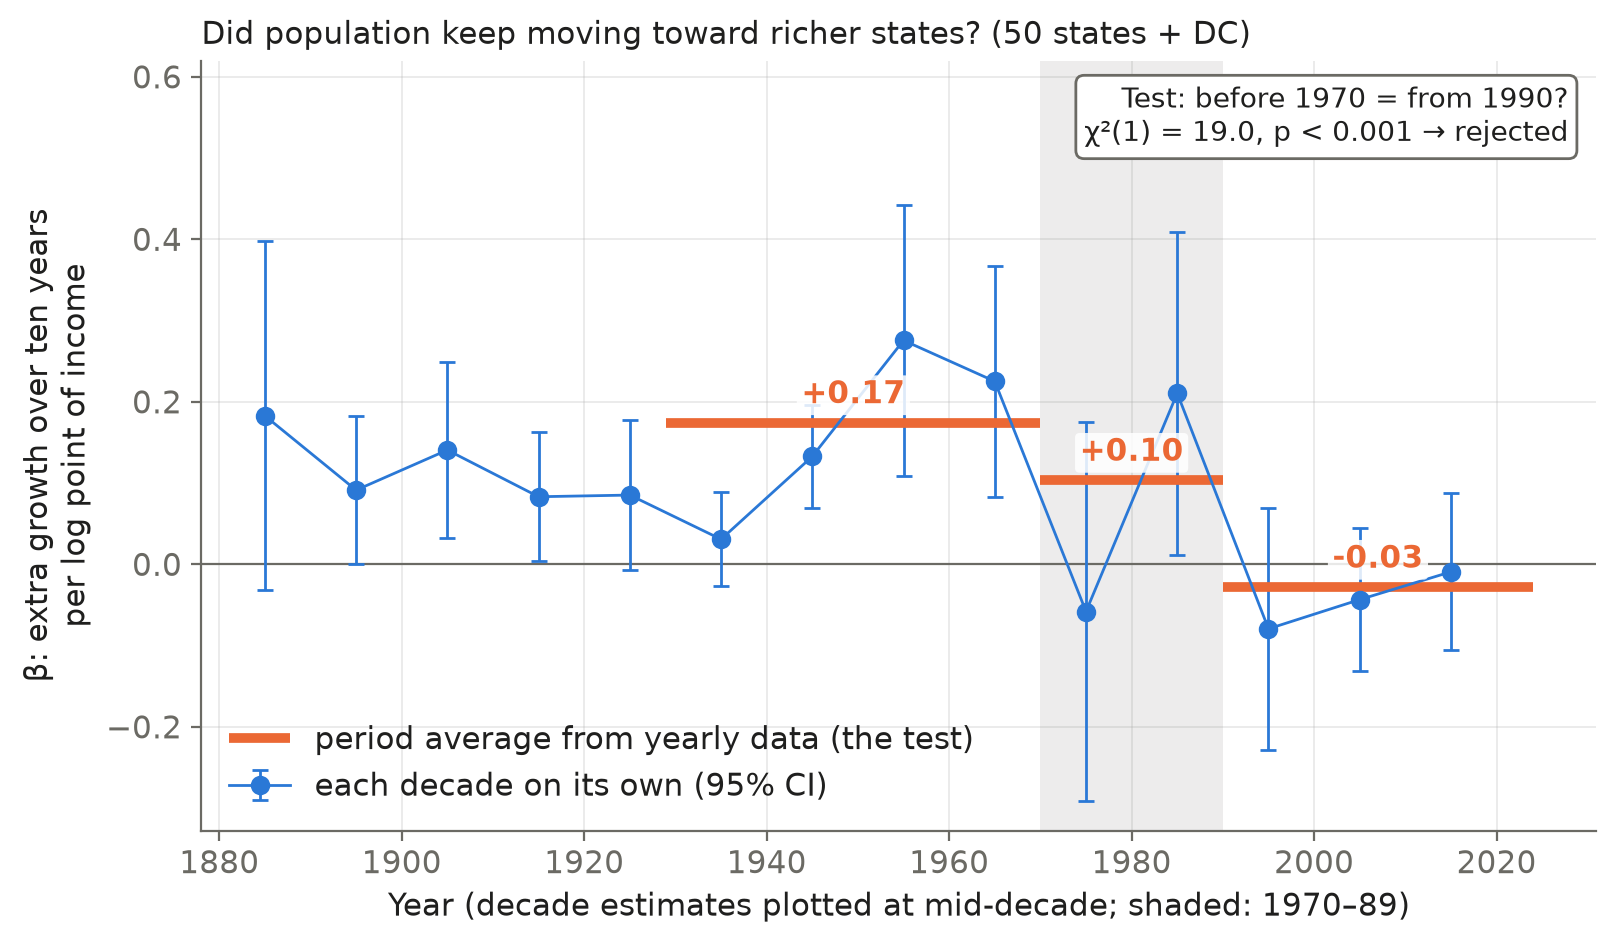
\includegraphics[width=\textwidth]{rq0b_test.png}
\caption{\textbf{Population growth toward richer states, 1880--2020.} Each \textbf{blue dot} is
the slope $\beta$ from equation~(\ref{eq:basic}), estimated on one decade alone (45 to 51 states;
all 51 from 1950), plotted at the middle of the decade, with a 95\% confidence interval. The three
\textbf{orange bars} are the period slopes from the test model, equation~(\ref{eq:test}), using
yearly data. The grey band marks 1970--89. The box reports the test of whether the first and last
orange bars are equal, and the $p$-value of the search over all break years.}
\label{fig:test}
\end{figure}

\paragraph{How to read Figure~\ref{fig:test}.} The vertical axis shows how much faster a richer
state grew. Points above the zero line mean that population grew faster where incomes were higher;
points near zero mean that income no longer predicted growth. From 1880 to the 1960s, every
decade's estimate is above zero, between 0.03 and 0.28, although several of the early intervals
include zero. In the 1970s the dot falls below zero, it rises again in the 1980s, and from the 1990s
on every dot is at or below zero. The orange bars summarize this: $+0.17$ before 1970, $+0.10$ in
1970--89 and $-0.03$ from 1990. Some decades have wide intervals because each blue dot uses only 45
to 51 data points, which is why the test pools many years.

\paragraph{Test result.} Table~\ref{tab:test} gives the estimates. The slope fell by 0.20 (95\%
confidence interval 0.11 to 0.29), with $W = 19.0$ and a nominal $p = 1.3 \times 10^{-5}$. Because
the cut years were chosen from these data, that $p$-value is too small. The sup-Wald test, which
searches over every break year, finds the best single break at 1990 with a statistic of 17.8,
against a 1\% critical value of 12.5. Its $p$-value, which accounts for the search, is 0.0008.
\textbf{We reject $H_0$ either way}: the link between income and growth before 1970 differs from the
link after 1990. In practical terms, a state with 10\% higher income grew about 1.7 percentage points
faster per decade before 1970. After 1990 the slope is $-0.03$ with a standard error of $0.05$, which
is not different from zero: income no longer predicted growth, but richer states did not clearly
grow \emph{slower}. This matches the direction Ganong and Shoag \cite{ganong} found with different
methods; they date the weakening to about 1980.

\begin{table}[htbp]
\centering\small
\caption{The test: income slope by period (yearly state data, 1929--2024; slopes on the
ten-year scale; standard errors clustered by state).}
\label{tab:test}
\begin{tabular}{lrr}
\toprule
& Estimate & Std.\ error \\
\midrule
$\hat\beta_{\text{before}}$ (1929--1969) & 0.174 & 0.038 \\
$\hat\beta_{\text{middle}}$ (1970--1989) & 0.103 & 0.112 \\
$\hat\beta_{\text{after}}$ (1990--2023)  & $-0.028$ & 0.047 \\
\midrule
Difference, before $-$ after & 0.203 & 0.046 \\
95\% confidence interval & \multicolumn{2}{r}{0.112 to 0.294} \\
Wald statistic $W$ ($\chi^2$, 1 d.f.) & \multicolumn{2}{r}{19.0} \\
$p$-value (nominal: cut years chosen from the data) & \multicolumn{2}{r}{$1.3\times10^{-5}$} \\
\midrule
Search over all break years: sup-Wald (best year 1990) & \multicolumn{2}{r}{17.8} \\
\quad critical values, 5\% / 1\% & \multicolumn{2}{r}{8.8 / 12.5} \\
\quad $p$-value, accounting for the search & \multicolumn{2}{r}{0.0008} \\
\midrule
Observations (state-years) / clusters (states) & \multicolumn{2}{r}{4,803 / 51} \\
\bottomrule
\end{tabular}
\end{table}

\paragraph{Is the result fragile?} I re-ran the test seven other ways. Each version changes the
assumptions in one area, and the test rejects $H_0$ in all of them, with the largest $p$-value
0.008 (Table~\ref{tab:robust}). The notebook's main version for dating the change adds separate year
effects for mining- and energy-producing states during the oil boom and bust; this report uses the
simpler version with year effects only, and the two give the same $p$-value.

\begin{table}[htbp]
\centering\small
\caption{The same test under other assumptions (nominal $p$-values).}
\label{tab:robust}
\begin{tabular}{>{\raggedright\arraybackslash}p{0.66\textwidth}r}
\toprule
Version & $p$-value \\
\midrule
This report's version (year effects only) & $1.3\times10^{-5}$ \\
Energy-producing states get their own year effects in 1973--1990 (oil boom and bust) & $1.3\times10^{-5}$ \\
\quad \ldots same, with a hand-picked list of energy states & $1.2\times10^{-5}$ \\
\quad \ldots same, oil years 1973--1986 only & $1.3\times10^{-5}$ \\
States compared only within their census division (9 regions) & 0.008 \\
Income standardized within each year (with energy-state year effects) & $4.9\times10^{-8}$ \\
World War II years (1940--46) left out (with energy-state year effects) & $2.2\times10^{-4}$ \\
Each state left out in turn (51 versions; largest $p$ shown) & $1.7\times10^{-4}$ \\
\bottomrule
\end{tabular}
\end{table}

\paragraph{When did it change?} The test establishes that a change happened, not when. The
middle period, 1970--89, is not significantly different from either side ($p = 0.42$ against
``before'' and $p = 0.16$ against ``after''). The decade dots show why: the 1970s look like the
period after, while in the 1980s growth again followed income. The project's rule for dating the
change, fixed in advance, gives no answer with the yearly data. With decade data it gives 1970, but
that answer depends on a single unit: leaving out the District of Columbia turns it into a gradual
change (and the yearly answer into 1990), while leaving out any other state changes nothing. DC is unusual, a city with no suburbs
inside its border. The timing is therefore still open.

\paragraph{Most of the change is in net migration.} Table~\ref{tab:split} splits the decade slopes
into net migration and the rest. These slopes are not on the same scale as Table~\ref{tab:test}:
they use decade data from 1950, so ``before'' means the 1950s--60s only, when the slope was highest,
and they use percent change. Of the 0.37 drop in the total slope between the 1950s--60s and the
1990s--2010s, 0.35 is in estimated net migration. Births and deaths followed income only weakly in
every period, and their slope did not change significantly ($p = 0.65$). The decade result is the
same without the six main immigrant gateway states (California, New York, New Jersey, Illinois,
Florida and Texas).

\begin{table}[htbp]
\centering\small
\caption{Income slope of decade growth and its two parts (50 states and DC; ten-year percent change;
the slopes add up exactly: total = net migration + the rest).}
\label{tab:split}
\begin{tabular}{lrrr}
\toprule
& 1950s--60s & 1970s--80s & 1990s--2010s \\
\midrule
Total growth & 0.320 & 0.096 & $-0.047$ \\
\quad Net migration (residual estimates) & 0.291 & 0.065 & $-0.058$ \\
\quad Births $-$ deaths (+ census coverage change) & 0.029 & 0.031 & 0.012 \\
\bottomrule
\end{tabular}
\end{table}

% -----------------------------------------------------------------------------
\subsection{Big cities: city first, whole metros later (Q2)}
\label{sec:cities}

\begin{figure}[htbp]
\centering
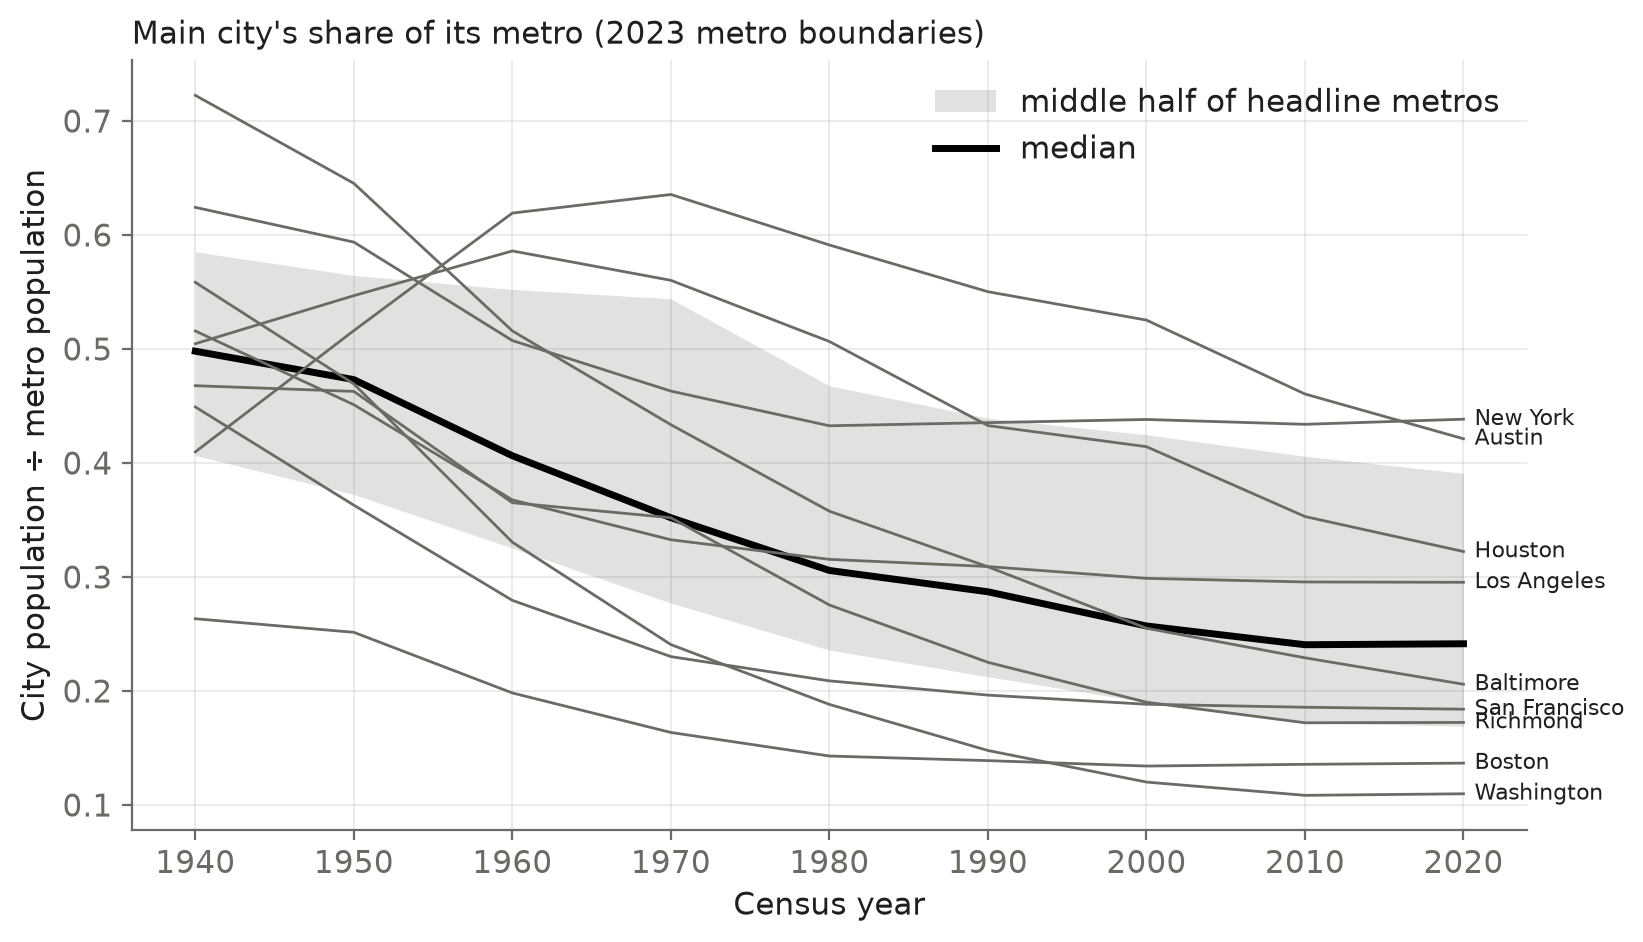
\includegraphics[width=\textwidth]{rq0a_city_share.png}
\caption{\textbf{The main city's share of its metro's population, 1940--2020.} Each thin grey line
is one of nine featured metros, labelled at the right. The \textbf{black line} is the median across
all 81 metros (the ``headline'' metros: those with a 1950 top-100 city), and the \textbf{grey band} holds the middle half of them (25th to 75th percentile).
Metro boundaries are the 2023 definitions throughout, so a falling share means the city grew more
slowly than the rest of its region, not that the region was redrawn.}
\label{fig:share}
\end{figure}

\paragraph{How to read Figure~\ref{fig:share}.} A value of 0.5 means half the metro lived in the
main city. In 1940 the typical big city held about half its metro's population; by 2020 it held
about a quarter. The fall is steepest between 1950 and 1980 and flattens after 2000. The share can
fall either because the city lost people or because the suburbs grew faster, so this figure alone
can't separate decline from suburbanization. Figure~\ref{fig:classes} does. Cities that annexed land,
such as Houston and Austin, kept a higher share for longer.

\begin{figure}[htbp]
\centering
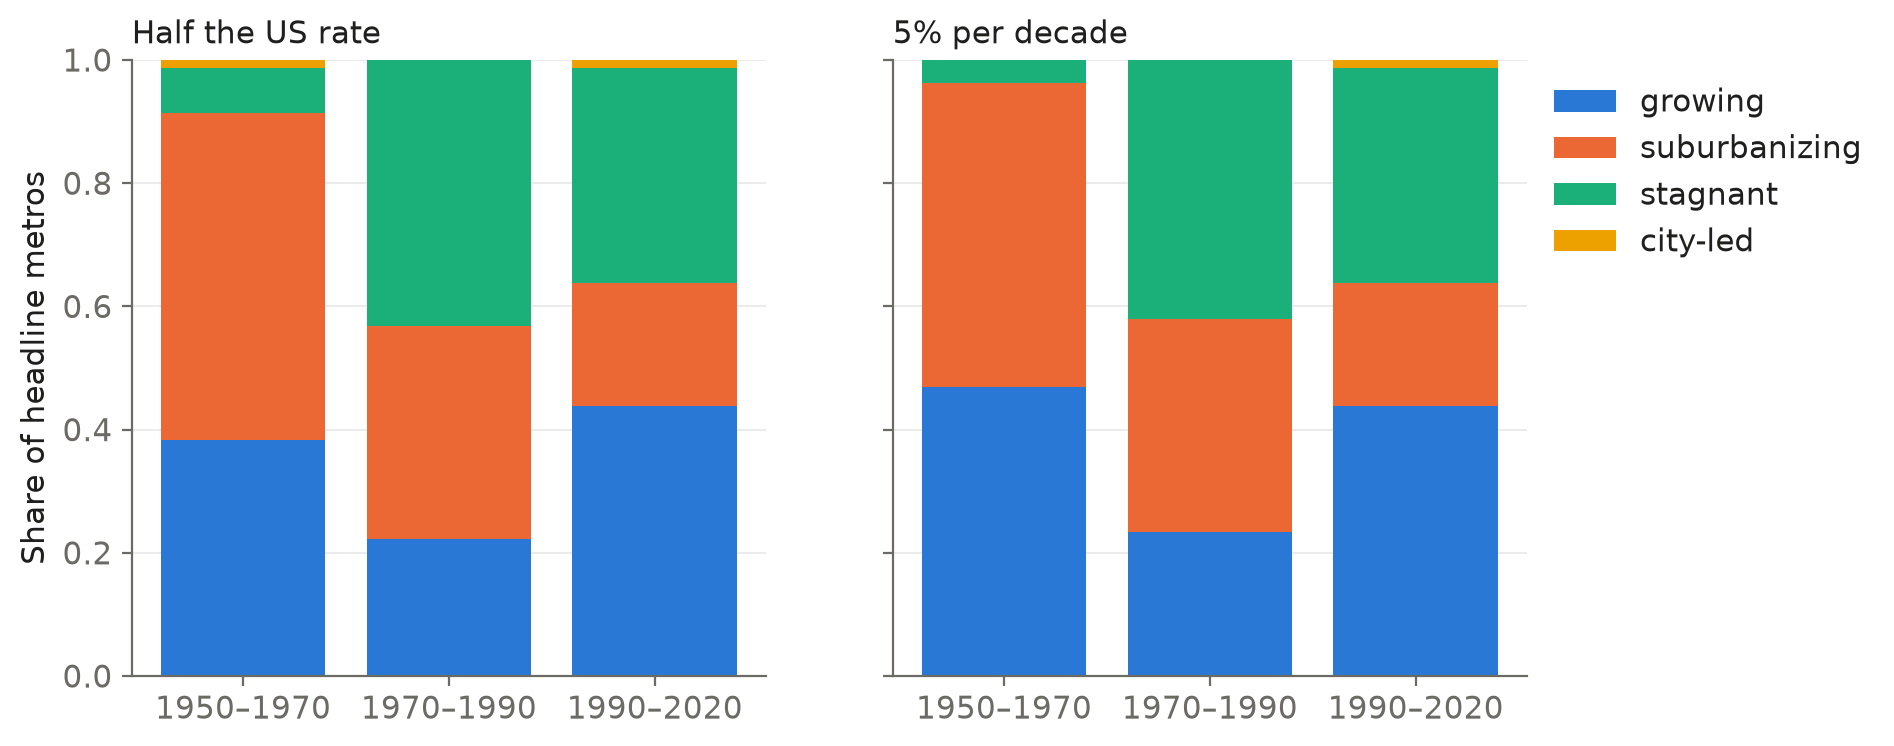
\includegraphics[width=\textwidth]{rq0a_classes.png}
\caption{\textbf{How the 81 big-city (``headline'') metros grew, by period.} Each bar divides the metros
into the four classes defined in Section~\ref{sec:citymetro}; the legend repeats the definitions.
Bar heights are shares, so each bar sums to 1. In 1990--2020 one metro (Denver) has no class,
because a county split across its boundary, so that bar covers 80 metros. \textbf{Left:} ``kept up''
means growth of at least half the US rate over the period (the main definition). \textbf{Right:}
``kept up'' means at least 5\% per decade, a fixed bar that does not depend on how fast the US grew
(a check).}
\label{fig:classes}
\end{figure}

\paragraph{How to read Figure~\ref{fig:classes}.} Read the colors from the bottom up. In
1950--70 (left panel), the largest group is orange, \emph{suburbanizing}: 43 of 81 metros (53\%)
kept up while their main city fell behind. Green, \emph{stagnant} (the whole metro fell
behind), is only 6 metros. In 1970--90 green becomes the largest group, 35 of 81 (43\%). In
1990--2020 it shrinks a little, to 28 of 80, while blue (\emph{growing}, city and metro both kept
up) recovers. The right panel, with a fixed 5\%-per-decade bar, shows a similar pattern, although
there suburbanizing and growing are nearly tied in 1950--70.

\paragraph{Results, with 90\% bootstrap ranges.}
\begin{itemize}
  \item \textbf{Mostly suburbanization in 1950--70, for cities that fell well behind.} Of the 49
        cities that fell behind, 88\% (79--96\%) were in metros that kept up; 33 of the 49 lost
        population. The share is 78--93\% under the alternative definitions fixed in advance. Stricter
        bars, tried afterwards, weaken it: 65\% (54--75\%) when ``kept up'' means three-quarters of US
        growth, and 52\% (41--63\%) at the full US rate. So the result holds for cities that fell
        well behind the US, not for every city that grew more slowly than the US.
  \item \textbf{Fixed-boundary cities fell behind far more often.} Among metros that kept up in
        1950--70, 30 of 33 fixed-boundary cities (91\%) fell behind, against 8 of 36 annexing cities
        (22\%); 5 cities with unknown land area are left out. The difference is 0.69 (0.54--0.82).
        Part of this is built in, since people in annexed land count as city growth.
  \item \textbf{Whole metros fell behind later.} The share of metros that fell behind rose from 9\%
        (1950--70) to 43\% (1970--90), then 36\% (1990--2020). The rise is 0.35 (0.25--0.44), and it
        holds at the stricter bars too. It is almost all in the Northeast and Midwest
        (12\% $\to$ 77\% $\to$ 61\%); in the South and West it stayed at 5--8\%. This pattern belongs
        to the old big metros: across all other US metros the share was 19\%, 21\% and 26\%. So
        choosing the 1950 top 100 makes the rise larger, not smaller.
\end{itemize}

% =============================================================================
\section{Limitations}

\begin{itemize}
  \item \textbf{Association, not cause.} The test shows that the link between income and growth
        changed. It does not show \emph{why}. Housing costs are one explanation; others include
        retirement migration to the Sun Belt, air conditioning, and the decline of manufacturing,
        which the regional pattern in Section~\ref{sec:cities} suggests: the Northeast and Midwest
        were hit hardest.
  \item \textbf{Timing.} The data agree that the change happened, but not on when. The decade
        answer of 1970 depends on whether DC is included.
  \item \textbf{States only.} The test uses states. The yearly break search on metro areas finds no
        significant break, but metro income data start only in 1969, too late to see a change around
        1970. Decade-level break tests on states, with only 51 data points per decade, find no break in
        their main version either; they do find one when income is standardized within each decade.
  \item \textbf{Equal weights.} Every state counts equally in the regressions, whatever its size;
        a population-weighted version has not been run.
  \item \textbf{Net migration is estimated}, not counted, and includes immigration from abroad.
  \item \textbf{Income data before 1929} come from historical estimates (Klein; Easterlin) that are
        less precise than BEA's; the test itself uses only BEA data from 1929. Income is not adjusted
        for differences in living costs between states.
  \item \textbf{Fixed 2023 metro boundaries} include counties that were rural in 1950. Using only
        the central counties changes the 1950--70 share by one metro (86\% instead of 88\%) and leaves
        all three answers the same.
  \item \textbf{Land areas} come from two sources that measure slightly differently (1950--80 and
        1990--2020), which adds some noise to the annexing classification.
\end{itemize}

% =============================================================================
\section{Next steps}

\begin{enumerate}
  \item Test the housing explanation directly: do metros that permit less housing (Census Building
        Permits Survey) or have stricter land-use rules (Wharton index) attract fewer people for the
        same income growth, and have their prices risen faster relative to income?
  \item Compare with other countries (OECD metro data), to see whether the US is unusual.
  \item A case study of a policy change: Auckland's 2016 upzoning and the construction that
        followed.
\end{enumerate}

% =============================================================================
\section*{Use of AI tools}
This report was written with the help of Claude Code, an AI coding assistant made by Anthropic.
It was used to write and test the data pipeline and analysis code, to make the figures and to
draft the text of this report. Three independent AI reviewers then checked the notebooks and this
report against the data; their corrections, mainly to how strongly the results were worded, are
included in this version.

% =============================================================================
\section*{Reproducibility}
The project is a Python package with a data pipeline, two analysis notebooks
(\nolinkurl{1.1-lr-us-structural-break} for Q1, \nolinkurl{1.0-lr-city-vs-metro} for Q2) and 249
automated tests that check both the code and the data, for example that city populations match
published Census figures. Every number in this report comes from, or is counted from, tables that
the notebooks write to \texttt{reports/tables/}.

% =============================================================================
\begin{thebibliography}{9}\small
\bibitem{andrews}
Andrews, D.~W.~K. (1993). Tests for parameter instability and structural change with unknown change
point. \emph{Econometrica}, 61(4), 821--856.
\bibitem{easterlin}
Easterlin, R.~A. (1957). State income estimates. In E.~S.~Lee, A.~R.~Miller, C.~P.~Brainerd and
R.~A.~Easterlin, \emph{Population Redistribution and Economic Growth, United States, 1870--1950},
Vol.~I. American Philosophical Society.
\bibitem{ganong}
Ganong, P., and Shoag, D. (2017). Why has regional income convergence in the U.S.\ declined?
\emph{Journal of Urban Economics}, 102, 76--90.
\bibitem{gibson}
Gibson, C. (1998). Population of the 100 largest cities and other urban places in the United
States: 1790 to 1990. US Census Bureau, Population Division Working Paper No.~27.
\bibitem{klein}
Klein, A. (2013). New state-level estimates of personal income in the United States, 1880--1910.
\emph{Research in Economic History}, 29. Figures taken from the working-paper version: Warwick
Economic Research Papers No.~916 (2009).
\bibitem{nhgis}
Manson, S., et al. IPUMS National Historical Geographic Information System. Minneapolis, MN:
IPUMS, University of Minnesota. \url{https://www.nhgis.org}
\bibitem{cesta}
Stanford Center for Spatial and Textual Analysis (CESTA). Historical U.S. city populations,
1790--2010. \url{https://github.com/cestastanford/historical-us-city-populations}
\bibitem{apl}
Winkler, R., Johnson, K.~M., et al. County-specific net migration estimates, 1950--2020. Applied
Population Laboratory, University of Wisconsin--Madison. \url{https://netmigration.wisc.edu}
\end{thebibliography}

\end{document}
